\documentclass{article}

\usepackage[preprint]{neurips_2025}
\usepackage[utf8]{inputenc}
\usepackage[T1]{fontenc}
\usepackage{hyperref}
\usepackage{url}
\usepackage{booktabs}
\usepackage{amsfonts}
\usepackage{amsmath}
\usepackage{nicefrac}
\usepackage{microtype}
\usepackage{xcolor}
\usepackage{graphicx}
\usepackage{subcaption}
\usepackage{array}
\usepackage{enumitem}
\usepackage{tabularx}
\usepackage{float}
\usepackage{placeins}

\newcommand{\needupdate}[1]{\textcolor{red}{#1}}
\newcommand{\figtodo}[1]{\fbox{\parbox{0.92\linewidth}{\centering\vspace{0.3cm}\textcolor{red}{#1}\vspace{0.3cm}}}}

\title{ReGraph-VLM: Cross-Subject Brain Graph and Vision Alignment for Natural-Image fMRI}

\author{%
  Anonymous Author(s)
}

\begin{document}

\maketitle

\begin{abstract}
Learning brain representations that generalize across subjects is a central challenge for connecting visual neuroscience with machine learning. We study repeated natural-image fMRI responses from the Natural Scenes Dataset using fixed-order HCP-MMP ROI graphs. We propose \textbf{Gated ReGraph-VLM}, a graph--vision model that encodes trial-level ROI response graphs with a fixed-order ROI transformer, applies a gated anatomy-preserving readout, and aligns brain graph embeddings with CLIP image embeddings. The main task is cross-subject same-image brain graph matching: given brain responses from different subjects, the model must identify whether they correspond to the same visual stimulus and retrieve the matching image or brain representation. Across all 8 held-out-subject folds and 3 random seeds, Gated ReGraph-VLM improves over ROI-MLP+CLIP on AUROC, AUPRC, Recall@5, MRR, image retrieval, and brain retrieval. It also remains strongest under hard-negative evaluation, preserves its advantage over ROI-MLP+CLIP in a stricter single-reference session-matched control, and outperforms task-matched decoding component baselines inspired by MindEye2-style shared ROI mapping, UMBRAE-style subject conditioning, and MindLink-style subject-adversarial training.

A rigorous set of new ablations changes the interpretation of the graph component. A no-adjacency gated ROI Transformer is statistically indistinguishable from the final BNT/ReGraph ROI-token variant, while ROI-order shuffling collapses performance and uniform or random gates substantially reduce performance. Static adjacency perturbations and learned edge-bias follow-ups do not improve over the no-adjacency gated ROI Transformer. These results show that the key inductive bias is not explicit fixed Pearson adjacency, but fixed anatomical ROI-token layout, learned transformer interactions, gated ROI-preserving readout, and image alignment. Held-out-image experiments further show that random image embeddings remain competitive for pair discrimination but collapse on image/brain retrieval, supporting the role of real CLIP semantics for unseen-image retrieval. Interpretability analyses show stable visual-ROI gates and strong functional importance under matched ROI deletion tests, while confound controls suggest that simple gate--repetition correlations should be interpreted cautiously. Together, these results support a fixed-order ROI-token Transformer-VLM framework for subject-invariant natural-image fMRI retrieval.
\end{abstract}

\section{Introduction}

Human responses to a natural image are not static. Across repeated presentations, visual cortex may preserve image-specific information while changing response magnitude and inter-regional structure due to adaptation, familiarity, memory, or session dynamics. The central scientific question of this project is whether a brain graph representation can capture the common image-driven component of fMRI responses across repetitions and across subjects.

We use NSD \citep{allen2022nsd}, a 7T fMRI dataset in which eight subjects viewed repeated natural scenes. For each trial-level response, we construct a graph
\begin{equation}
  G_{s,i,r} = (V, A, X_{s,i,r}),
\end{equation}
where $s$ is subject, $i$ is image, $r \in \{1,2,3\}$ is ordinal repetition index, $V$ is a fixed set of 180 HCP-MMP ROIs \citep{glasser2016mmp}, $X_{s,i,r}\in\mathbb{R}^{180\times4}$ contains scalar ROI beta-response summaries, and $A$ is a training-derived ROI adjacency.

The project originally began with static atlas ROI graph classification and BrainGNN-style baselines. Those experiments were useful for validating the graph construction pipeline, but static 766-way image identity classification was too difficult for compressed ROI summaries and did not yield a convincing graph advantage. We therefore shifted to a neuroscience-driven setting: repeated natural-image responses. The strongest final task is now \emph{cross-subject same-image brain graph retrieval}. This task asks whether a shared model can map different subjects' brain graph responses to the same image into a common embedding space.

Figure~\ref{fig:model} summarizes the current final model. ReGraph-VLM combines a fixed-order ROI graph transformer, a gated ROI-preserving readout, and CLIP-style image alignment. The fixed-order graph encoder uses the fact that HCP-MMP ROI identity is anatomically meaningful and aligned across subjects. The VLM branch provides an image-level embedding anchor for brain-image retrieval. The final ablations show that the explicit fixed adjacency matrix is not the main driver of the improvement; the useful structure is the fixed anatomical ROI-token layout with learned transformer interactions and gated readout.

\begin{figure}[!htbp]
  \centering
  \IfFileExists{figures/model_overview.pdf}{%
    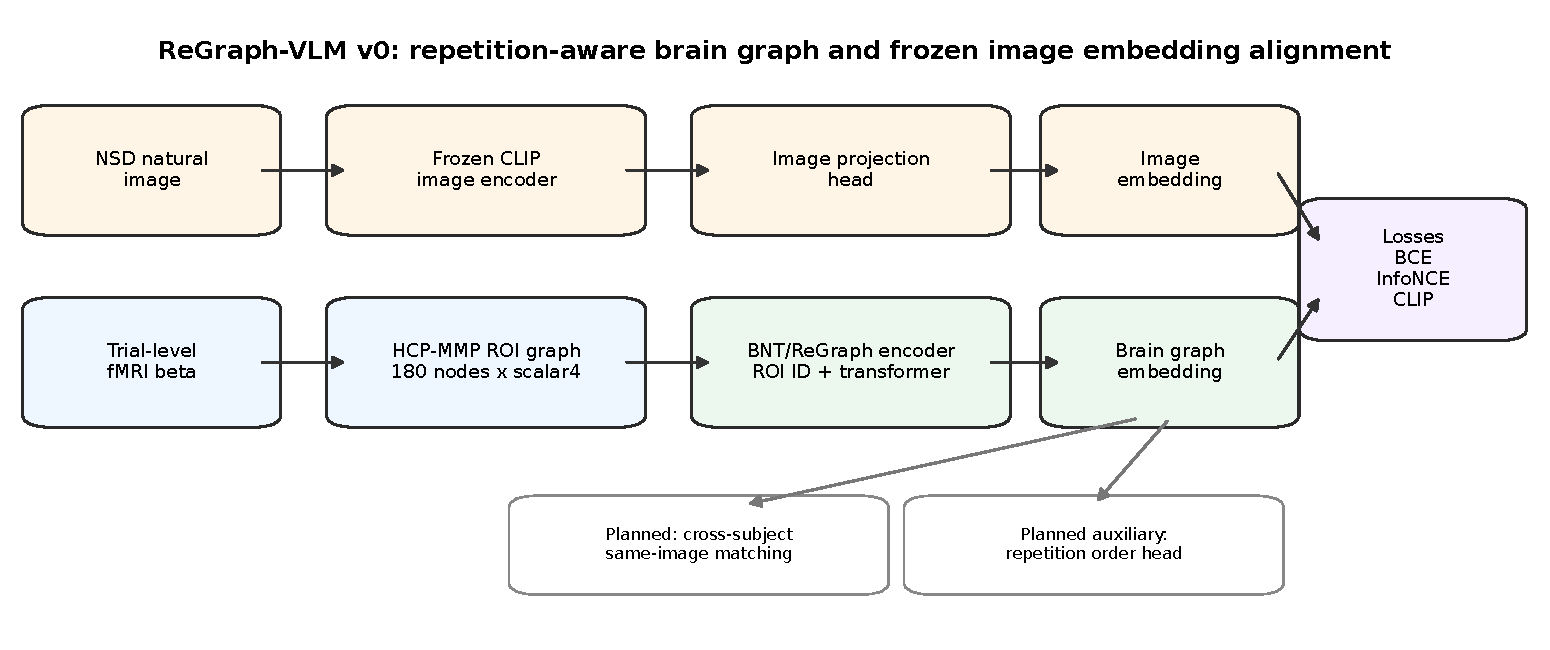
\includegraphics[width=0.98\linewidth]{figures/model_overview.pdf}%
  }{%
    \figtodo{Upload/update \texttt{figures/model\_overview.pdf}: ReGraph-VLM model diagram showing ROI graph encoder, gated-flatten readout, frozen CLIP image encoder, and cross-subject retrieval objective.}%
  }
  \caption{ReGraph-VLM overview.}
  \label{fig:model}
\end{figure}

\section{Data, Graph Construction, and Tasks}

\paragraph{Atlas ROI graph.}
We pivoted from learned shared-unit graphs to atlas ROI graphs. Each node is one HCP-MMP cortical parcel, yielding 180 fixed-order nodes. This fixed node order is important: unlike generic graphs, ROI identity is anatomically meaningful, so readouts that destroy ROI position can fail.

\paragraph{Node features.}
For each ROI and trial-level beta response, we compute four scalar features:
\begin{equation}
  X_i = [\mathrm{mean\ beta},\ \mathrm{std\ beta},\ q90\ \mathrm{beta},\ \mathrm{positive\ fraction}].
\end{equation}
This feature set is intentionally simple. It allowed stable dataset construction and produced a strong ROI MLP sanity baseline.

\paragraph{Strict T=3 repetition dataset.}
We use strict three-repeat sequences, so each usable sample contains $(G_{s,i,1}, G_{s,i,2}, G_{s,i,3})$. Dataset QC confirmed that strict T=3 is feasible, that trial-level scalar4 caches are valid, and that NaN/Inf counts are zero. Each strict T=3 sequence gives three same-image repeat pairs: repeat 1--2, repeat 1--3, and repeat 2--3.

\paragraph{Within-subject repeat matching.}
The first modeling task pairs repeated graphs from the same subject and same image as positives. Negatives are same-subject and repeat-pair matched but use different images. This task validates whether an embedding preserves image-specific information across repeated presentations within one person.

\paragraph{Cross-subject same-image matching.}
The final main task pairs graphs from different subjects who viewed the same image. A positive pair has the same image and matched repeat index but different subjects; a negative pair has different images and different subjects. The key retrieval setting asks whether a held-out subject's brain graph can retrieve the matching image or the corresponding brain graph from other subjects. This is the strongest task because it tests whether the model learns a shared, subject-invariant brain graph representation.

\paragraph{Split accounting and leakage checks.}
For the main all-fold cross-subject setting, each fold holds out one subject for testing and uses only training-fold data to construct model inputs such as adjacency. Table~\ref{tab:split_accounting} reports the serialized pair counts used by the final audit. No fold has train--test subject overlap. For held-out-image checks, the train--test NSD image-overlap rate is 0 in the audited folds.

\begin{table}[!htbp]
  \centering
  \caption{Final split accounting for the main cross-subject all-fold dataset. Sequence counts are strict T=3 image sequences; pair counts include one positive and one matched negative per anchor trial. Hard-negative all-fold splits use the same fold-level anchor counts.}
  \label{tab:split_accounting}
  \scriptsize
  \setlength{\tabcolsep}{3.2pt}
  \renewcommand{\arraystretch}{1.12}
  \begin{tabular}{lllrrrrrrr}
    \toprule
    Fold & Test subj. & Val subj. & Train seq. & Val seq. & Test seq. & Train pairs & Val pairs & Test pairs & Test imgs \\
    \midrule
    fold\_01 & subj01 & subj08 & 3975 & 515 & 766 & 23850 & 3090 & 4596 & 766 \\
    fold\_02 & subj02 & subj08 & 3975 & 515 & 766 & 23850 & 3090 & 4596 & 766 \\
    fold\_03 & subj03 & subj08 & 4160 & 515 & 581 & 24960 & 3090 & 3486 & 581 \\
    fold\_04 & subj04 & subj08 & 4226 & 515 & 515 & 25356 & 3090 & 3090 & 515 \\
    fold\_05 & subj05 & subj08 & 3975 & 515 & 766 & 23850 & 3090 & 4596 & 766 \\
    fold\_06 & subj06 & subj08 & 4160 & 515 & 581 & 24960 & 3090 & 3486 & 581 \\
    fold\_07 & subj07 & subj08 & 3975 & 515 & 766 & 23850 & 3090 & 4596 & 766 \\
    fold\_08 & subj08 & subj07 & 3975 & 766 & 515 & 23850 & 4596 & 3090 & 515 \\
    \bottomrule
  \end{tabular}
\end{table}

\paragraph{Anchor-side session/order matching.}
We also audited the serialized cross-subject pair tensors for session/order confounds. For every anchor trial, pair construction creates one positive and one negative example using the same anchor brain response. Thus, the positive and negative examples should share anchor subject, anchor image, repeat index, and anchor session. Table~\ref{tab:session_order_pair_qc} confirms this exactly for all train, validation, and test pairs. This is an anchor-side session/order control; the reference side is an average over training-subject responses and therefore does not define a single reference session. We therefore add a stricter single-reference session-matched evaluation in Section~\ref{sec:single_ref_control}.

\begin{table}[!htbp]
  \centering
  \caption{Session/order QC for the serialized main cross-subject pair tensors. Each complete anchor group contains one positive and one negative generated from the same anchor trial.}
  \label{tab:session_order_pair_qc}
  \scriptsize
  \setlength{\tabcolsep}{4pt}
  \renewcommand{\arraystretch}{1.15}
  \begin{tabular}{lrrrrrr}
    \toprule
    Split & Pairs & Pos. & Neg. & Complete groups & Problem groups & Anchor match \\
    \midrule
    Train & 194526 & 97263 & 97263 & 97263 & 0 & 100\% \\
    Val & 26226 & 13113 & 13113 & 13113 & 0 & 100\% \\
    Test & 31536 & 15768 & 15768 & 15768 & 0 & 100\% \\
    All & 252288 & 126144 & 126144 & 126144 & 0 & 100\% \\
    \bottomrule
  \end{tabular}
\end{table}

\section{Completed Neuroscience Analyses}

Before training graph models, we tested whether repetition/familiarity signals are present in the ROI graphs. Figure~\ref{fig:neuro} summarizes the completed analyses.

\begin{figure}[!htbp]
  \centering
  \IfFileExists{figures/neuroscience_summary.pdf}{%
    
\includegraphics[width=0.8\linewidth]{figures/neuroscience_summary.pdf}%
  }{%
    \figtodo{Upload/update \texttt{figures/neuroscience\_summary.pdf}: ROI repetition effects, same-vs-different repeat similarity, and graph reconfiguration summary.}%
  }
  \caption{Neuroscience sanity checks for repeated natural-image brain graphs.
(a) Repeated viewing induces measurable ROI-level response changes, with more HCP-MMP ROIs showing FDR-significant effects for repeat3--repeat1 than repeat2--repeat1.
(b) Real repetition-related ROI response changes are substantially larger than shuffled repeat-label controls, indicating that the effect is not explained by random repeat assignment.
(c) Same-image repeated graphs are consistently more similar than different-image controls across all repeat pairs, supporting the presence of repeat-stable image-specific brain graph structure.
(d) Repeat-specific ROI correlation graphs remain globally stable, but local edge changes are measurable and are larger for repeat3--repeat1 than repeat2--repeat1.
}
  \label{fig:neuro}
\end{figure}

\paragraph{ROI repetition effects.}
Repeated viewing produced measurable ROI-level changes. We found 41 FDR-significant ROIs for repeat2-repeat1 and 56 FDR-significant ROIs for repeat3-repeat1. The mean absolute real effects were much larger than shuffled-repeat controls: 10.90 versus 2.56 for repeat2-repeat1, and 14.33 versus 2.48 for repeat3-repeat1. This supports the claim that trial-level ROI responses change systematically across repeated viewing, consistent with repetition suppression/enhancement phenomena \citep{grill2006repetition}.

\paragraph{Same-image representational stability.}
Same-image repeated graphs were consistently more similar than different-image controls. For repeat pairs 1--2, 1--3, and 2--3, same-image correlations were 0.8916, 0.8851, and 0.8871, respectively, compared with different-image correlations of 0.8305, 0.8296, and 0.8292. The same-minus-different gaps were therefore 0.0612, 0.0555, and 0.0579.

\paragraph{Graph reconfiguration.}
Repeat-specific ROI correlation matrices were globally stable across repetitions, but local edge-level changes existed. Train-only fold-consistent edge analysis found 9 repeat-sensitive edges, including 3 fold-consistent repeat2-repeat1 edges and 6 repeat3-repeat1 edges. We interpret this conservatively: repeated viewing does not globally rewire the ROI graph, but local edge changes may carry repetition information.

\section{Models}

\paragraph{Raw and non-graph baselines.}
The raw baseline scores pairs using Pearson correlation over flattened ROI features. The strongest non-graph learned baseline is a Siamese ROI MLP trained with BCE+InfoNCE. This baseline is important because it preserves fixed ROI order through flattening and directly optimizes repeat matching.

\paragraph{Graph baselines.}
We tested GCN, GAT, BrainGNN \citep{li2021braingnn}, and Brain Network Transformer (BNT) \citep{kan2022bnt}. Naive GCN and BrainGNN collapsed in the pair-retrieval setting. This does not imply that graph structure is useless; rather, standard graph pooling can destroy fixed anatomical ROI identity. BNT-token with ROI identity and flatten readout was much stronger than BrainGNN and competitive with the ROI MLP.

\paragraph{Task-matched decoding component baselines.}
To position ReGraph-VLM against recent fMRI-to-image and cross-subject decoding ideas, we added task-matched component baselines inspired by MindEye2, UMBRAE, and MindLink. These are not full image-reconstruction systems; instead, they adapt the core ideas most relevant to our retrieval task: shared ROI-to-image mapping, subject-conditioned universal encoding, and subject-adversarial training. This lets us test whether ReGraph-VLM remains useful against stronger decoding-style components beyond BrainGNN and BNT, while avoiding claims of full-system comparison.

\paragraph{ReGraph-VLM.}
The final model is Gated ReGraph-VLM. It uses a fixed-order BNT/ReGraph-style ROI token transformer as the brain branch and a frozen CLIP image encoder \citep{radford2021clip} as the image branch. The training objective combines pairwise BCE, repeat InfoNCE \citep{oord2018infonce}, and CLIP-style brain-image contrastive alignment:
\begin{equation}
  \mathcal{L} = \mathcal{L}_{\mathrm{BCE}} + \mathcal{L}_{\mathrm{repeat\ InfoNCE}} + \lambda_{\mathrm{clip}}\mathcal{L}_{\mathrm{CLIP}}.
\end{equation}
We use $\lambda_{\mathrm{clip}}=2.0$ in the final main runs.

\paragraph{Gated-flatten readout.}
The most important architecture change is the gated-flatten readout. Let $h_i$ be the final embedding of ROI $i$. The gated readout computes
\begin{equation}
  g_i = \sigma(\mathrm{MLP}_{\mathrm{gate}}(h_i)), \qquad \tilde{h}_i = g_i h_i,
\end{equation}
then flattens $[\tilde{h}_1,\ldots,\tilde{h}_{180}]$ and projects the result to the final brain embedding. This readout preserves the fixed ROI layout while allowing the model to emphasize task-relevant ROIs.

\subsection{Experimental protocol and implementation details}

For binary pair matching, the model predicts a logit $\ell_j$ for each pair in a minibatch and optimizes
\begin{equation}
  \mathcal{L}_{\mathrm{BCE}}
  = -\frac{1}{B}\sum_{j=1}^{B}
  y_j\log\sigma(\ell_j) + (1-y_j)\log(1-\sigma(\ell_j)).
\end{equation}
For repeat InfoNCE, we keep only positive same-image pairs in the minibatch, encode the two brain responses as $u_j$ and $v_j$, L2-normalize embeddings through the projection heads, and use other positive pairs in the minibatch as negatives:
\begin{equation}
  \mathcal{L}_{\mathrm{repeat\ InfoNCE}}
  = \frac{1}{2}\left[
  \mathrm{CE}\left(\frac{UV^\top}{\tau_{\mathrm{brain}}}, I\right)
  +
  \mathrm{CE}\left(\frac{VU^\top}{\tau_{\mathrm{brain}}}, I\right)
  \right].
\end{equation}
The CLIP alignment loss uses the same symmetric contrastive form between brain embeddings and frozen CLIP image embeddings from both sides of each pair. Let $B\in\mathbb{R}^{B\times d}$ be the L2-normalized projected brain embeddings in a minibatch and let $C\in\mathbb{R}^{B\times d}$ be the corresponding L2-normalized projected CLIP image embeddings. The positive index for each brain anchor is its paired image in the same minibatch, and all other images in the minibatch are negatives:
\begin{equation}
  \mathcal{L}_{\mathrm{CLIP}}
  = \frac{1}{2}\left[
  \mathrm{CE}\left(\frac{BC^\top}{\tau_{\mathrm{clip}}}, I\right)
  +
  \mathrm{CE}\left(\frac{CB^\top}{\tau_{\mathrm{clip}}}, I\right)
  \right].
\end{equation}
The final objective uses $\lambda_{\mathrm{clip}}=2.0$ unless otherwise stated.

The adjacency matrix is built from training data only for each fold. We use absolute ROI-response correlations, add diagonal self-connections, and apply symmetric degree normalization. Validation and test responses are never used to construct adjacency. Adjacency ablations replace this matrix with no-adjacency, identity, shuffled, random, top-$k$, or edge-dropped variants; these controls are used only to diagnose whether explicit fixed adjacency contributes beyond fixed ROI-token layout.

\begin{table}[!htbp]
  \centering
  \caption{Implementation and training details for the main ReGraph-VLM runs.}
  \label{tab:implementation_details}
  \scriptsize
  \setlength{\tabcolsep}{5pt}
  \renewcommand{\arraystretch}{1.15}
  \begin{tabularx}{\linewidth}{lX}
    \toprule
    Item & Setting \\
    \midrule
    Input graph & 180 fixed-order HCP-MMP ROIs; 4 scalar ROI beta-summary features per node \\
    Brain encoder & Fixed-order ROI-token transformer; hidden dimension 64; 2 layers; 4 heads; dropout 0.3 \\
    Readout & Flat or gated-flat ROI-preserving readout; final embedding dimension 128 \\
    Image branch & Frozen CLIP image embeddings with learned projection head to the shared 128-d space \\
    Loss & BCE + repeat InfoNCE + $\lambda_{\mathrm{clip}}$ CLIP alignment; $\lambda_{\mathrm{clip}}=2.0$ for final CLIP runs \\
    Temperatures & $\tau_{\mathrm{brain}}=0.1$ for repeat InfoNCE; $\tau_{\mathrm{clip}}=0.07$ for brain-image alignment \\
    Optimization & AdamW, learning rate $10^{-3}$, weight decay $10^{-4}$, batch size 128, gradient clipping at 5.0 \\
    Training protocol & Up to 80 epochs with patience 12; checkpoint selected by validation AUROC \\
    Evaluation & 8 held-out-subject folds and seeds 11, 22, and 33 for main all-fold summaries \\
    \bottomrule
  \end{tabularx}
\end{table}

\subsection{Evaluation metrics}

We separate pair discrimination from retrieval. AUROC and AUPRC are computed over binary same-image versus different-image pair scores. For retrieval metrics, each query has a candidate set $\mathcal{C}_q$ with one correct same-image target $c_q^\star$. If the target rank is $r_q$, then
\begin{equation}
  \mathrm{R@5}=\frac{1}{Q}\sum_{q=1}^{Q}\mathbf{1}[r_q\leq5],
  \qquad
  \mathrm{MRR}=\frac{1}{Q}\sum_{q=1}^{Q}\frac{1}{r_q}.
\end{equation}
Plain R@5/MRR use the model's pair score to rank candidate brain-pair matches. Image R@5 ranks candidate CLIP image embeddings for a query brain embedding. Brain R@5 and brain MRR rank candidate brain embeddings directly in the learned brain-embedding space. This distinction matters for held-out-image controls: random image anchors can remain competitive for pair discrimination, but should fail on image/brain retrieval if semantic image structure is required.

\section{Main Results}

\subsection{Within-subject same-image repeat matching}

Table~\ref{tab:within_subject} reports the completed within-subject repeat-matching results. The main result is a tradeoff: ROI MLP variants are stronger for binary same/different discrimination, while BNT/ReGraph variants are competitive on retrieval-style metrics.

\begin{table}[!htbp]
  \centering
  \caption{Within-subject same-image repeat matching results. Values are means over the available smoke folds and seeds for each experiment.}
  \label{tab:within_subject}
  \small
  \begin{tabular}{lcccc}
    \toprule
    Model & AUROC & AUPRC & R@5 & MRR \\
    \midrule
    Raw Pearson flat & 0.6182 & -- & 0.0522 & 0.0433 \\
    ROI MLP + BCE & 0.7672 & 0.7336 & 0.0543 & 0.0442 \\
    ROI MLP + BCE+InfoNCE & \textbf{0.7778} & \textbf{0.7540} & \textbf{0.0758} & \textbf{0.0592} \\
    Naive GCN & 0.5000 & -- & -- & -- \\
    BrainGNN Siamese & 0.5000 & -- & -- & -- \\
    BNT-token + BCE+InfoNCE & 0.7693 & 0.7512 & 0.0718 & 0.0584 \\
    \bottomrule
  \end{tabular}
\end{table}

\subsection{All-fold cross-subject matching}

The main final result is all-fold cross-subject same-image matching over 8 held-out-subject folds and 3 seeds. Gated ReGraph+CLIP improves over ROI-MLP+CLIP and flat ReGraph+CLIP on all listed metrics (Table~\ref{tab:cross_subject_main}). Paired tests over fold$\times$seed are strong for the comparison against ROI-MLP+CLIP: AUROC difference $+0.0095$ with $p=1.77\times10^{-5}$, AUPRC difference $+0.0168$ with $p=4.66\times10^{-8}$, R@5 difference $+0.0117$ with $p=2.85\times10^{-5}$, and brain R@5 difference $+0.0159$ with $p=2.98\times10^{-7}$.

\begin{table}[!htbp]
  \centering
  \caption{Main all-fold cross-subject results over 8 held-out-subject folds and 3 random seeds. Values are mean $\pm$ std over fold$\times$seed runs.}
  \label{tab:cross_subject_main}
  \scriptsize
  \setlength{\tabcolsep}{3.5pt}
  \renewcommand{\arraystretch}{1.15}
  \begin{tabular}{lcccccc}
    \toprule
    Model & AUROC & AUPRC & R@5 & MRR & Img R@5 & Brain R@5 \\
    \midrule
    ROI-MLP+CLIP
    & $0.8164{\scriptstyle\pm0.0518}$
    & $0.7896{\scriptstyle\pm0.0532}$
    & $0.0782{\scriptstyle\pm0.0273}$
    & $0.0636{\scriptstyle\pm0.0190}$
    & $0.0729{\scriptstyle\pm0.0280}$
    & $0.0837{\scriptstyle\pm0.0291}$ \\
    Flat ReGraph+CLIP
    & $0.8210{\scriptstyle\pm0.0481}$
    & $0.8022{\scriptstyle\pm0.0460}$
    & $0.0865{\scriptstyle\pm0.0318}$
    & $0.0677{\scriptstyle\pm0.0213}$
    & $0.0812{\scriptstyle\pm0.0305}$
    & $0.0966{\scriptstyle\pm0.0299}$ \\
    Gated ReGraph+CLIP
    & $\mathbf{0.8259}{\scriptstyle\pm0.0523}$
    & $\mathbf{0.8065}{\scriptstyle\pm0.0528}$
    & $\mathbf{0.0899}{\scriptstyle\pm0.0357}$
    & $\mathbf{0.0695}{\scriptstyle\pm0.0240}$
    & $\mathbf{0.0847}{\scriptstyle\pm0.0318}$
    & $\mathbf{0.0996}{\scriptstyle\pm0.0310}$ \\
    \bottomrule
  \end{tabular}
\end{table}

\subsection{Task-matched component baseline comparison}

We further compared Gated ReGraph+CLIP against several task-matched brain-decoding component baselines inspired by recent fMRI-to-image and cross-subject decoding methods. These baselines are not intended to reproduce full image-reconstruction pipelines; instead, they adapt the relevant representation-learning components to our cross-subject same-image retrieval setting. The comparison includes a MindEye2-style shared ROI mapper, an UMBRAE-style subject-conditioned encoder, and MindLink-style subject-adversarial variants. Table~\ref{tab:sota_baselines} shows that the previous final Gated ReGraph+CLIP model remains stronger than all submitted component baselines. The closest competitor is the MindLink-style subject-adversarial ROI-MLP, but it remains lower on every key metric.

\begin{table}[!htbp]
  \centering
  \caption{Task-matched decoding component baseline comparison on the cross-subject same-image matching task. Values are mean $\pm$ std over the available fold$\times$seed runs. These are not full image-reconstruction system comparisons.}
  \label{tab:sota_baselines}
  \scriptsize
  \setlength{\tabcolsep}{2.8pt}
  \renewcommand{\arraystretch}{1.15}
  \begin{tabular}{lccccccc}
    \toprule
    Model & $n$ & AUROC & AUPRC & R@5 & MRR & Img R@5 & Brain R@5 \\
    \midrule
    Our Gated ReGraph+CLIP
    & 24 & $\mathbf{0.8259{\scriptstyle\pm0.0413}}$ & $\mathbf{0.8065{\scriptstyle\pm0.0460}}$ & $\mathbf{0.0899{\scriptstyle\pm0.0356}}$ & $\mathbf{0.0695{\scriptstyle\pm0.0240}}$ & $\mathbf{0.0847{\scriptstyle\pm0.0357}}$ & $\mathbf{0.0996{\scriptstyle\pm0.0369}}$ \\
    MindEye2-style shared ROI mapper
    & 24 & $0.4982{\scriptstyle\pm0.0138}$ & $0.5006{\scriptstyle\pm0.0117}$ & $0.0078{\scriptstyle\pm0.0019}$ & $0.0111{\scriptstyle\pm0.0021}$ & $0.0080{\scriptstyle\pm0.0019}$ & $0.0086{\scriptstyle\pm0.0035}$ \\
    UMBRAE-style subject encoder
    & 24 & $0.7415{\scriptstyle\pm0.0678}$ & $0.7061{\scriptstyle\pm0.0645}$ & $0.0308{\scriptstyle\pm0.0105}$ & $0.0307{\scriptstyle\pm0.0086}$ & $0.0329{\scriptstyle\pm0.0131}$ & $0.0360{\scriptstyle\pm0.0161}$ \\
    MindLink-style subject-adversarial ROI-MLP
    & 24 & $0.8135{\scriptstyle\pm0.0555}$ & $0.7873{\scriptstyle\pm0.0575}$ & $0.0774{\scriptstyle\pm0.0306}$ & $0.0616{\scriptstyle\pm0.0206}$ & $0.0713{\scriptstyle\pm0.0290}$ & $0.0835{\scriptstyle\pm0.0335}$ \\
    MindLink-style subject-adversarial ReGraph
    & 8 & $0.5547{\scriptstyle\pm0.1070}$ & $0.5475{\scriptstyle\pm0.0957}$ & $0.0146{\scriptstyle\pm0.0122}$ & $0.0165{\scriptstyle\pm0.0104}$ & $0.0135{\scriptstyle\pm0.0155}$ & $0.0161{\scriptstyle\pm0.0221}$ \\
    \bottomrule
  \end{tabular}
\end{table}

The component-baseline comparison gives two useful diagnostics. First, simply sharing an ROI-to-image mapper is insufficient: the MindEye2-style shared ROI mapper collapses to chance, suggesting that our cross-subject graph task cannot be solved by a naive shared mapping. Second, subject conditioning and subject-adversarial training are not automatically beneficial. The UMBRAE-style subject encoder improves over chance but remains far behind Gated ReGraph+CLIP, while the MindLink-style adversarial ROI-MLP is the strongest component baseline but still lower on AUROC, retrieval R@5/MRR, and brain retrieval. Paired fold$\times$seed tests against this closest component baseline favor Gated ReGraph+CLIP for AUROC ($+0.0124$, $p=7.77\times10^{-4}$), R@5 ($+0.0125$, $p=9.39\times10^{-4}$), and brain R@5 ($+0.0160$, $p=6.91\times10^{-5}$). The adversarial ReGraph variant is unstable in this setting and was therefore kept as a seed-11 diagnostic rather than expanded further, indicating that subject-invariance objectives must be tuned carefully for fixed-order ROI graph transformers.

\subsection{Graph-only and CLIP alignment ablation}

The gated graph-only model performs reasonably for pair discrimination but has near-chance image/brain retrieval without CLIP alignment (Table~\ref{tab:graph_only}). This shows that the graph branch learns useful brain-brain matching, while the VLM branch is necessary for image-brain retrieval.

\begin{table}[!htbp]
  \centering
  \caption{Gated graph-only control over 8 held-out-subject folds and 3 random seeds. Values are mean $\pm$ std over fold$\times$seed runs.}
  \label{tab:graph_only}
  \scriptsize
  \setlength{\tabcolsep}{3.5pt}
  \renewcommand{\arraystretch}{1.15}
  \begin{tabular}{lcccccc}
    \toprule
    Model & AUROC & AUPRC & R@5 & MRR & Img R@5 & Brain R@5 \\
    \midrule
    Gated ReGraph
    & $0.8192{\scriptstyle\pm0.0502}$
    & $0.7940{\scriptstyle\pm0.0510}$
    & $0.0802{\scriptstyle\pm0.0322}$
    & $0.0639{\scriptstyle\pm0.0213}$
    & $0.0075{\scriptstyle\pm0.0028}$
    & $0.0075{\scriptstyle\pm0.0022}$ \\
    Gated ReGraph + CLIP
    & $\mathbf{0.8259}{\scriptstyle\pm0.0413}$
    & $\mathbf{0.8065}{\scriptstyle\pm0.0460}$
    & $\mathbf{0.0899}{\scriptstyle\pm0.0356}$
    & $\mathbf{0.0695}{\scriptstyle\pm0.0240}$
    & $\mathbf{0.0847}{\scriptstyle\pm0.0357}$
    & $\mathbf{0.0996}{\scriptstyle\pm0.0369}$ \\
    \bottomrule
  \end{tabular}
\end{table}

\subsection{Adjacency and ROI-token ablations}

The improvement over ROI-MLP+CLIP is real, but new ablations show that it does not come from explicit fixed adjacency. A no-adjacency gated ROI Transformer is statistically indistinguishable from the final BNT/ReGraph ROI-token variant, and explicit graph-biased variants do not improve over it. The stronger conclusion is that fixed ROI-token layout, transformer interactions, gated readout, and CLIP alignment drive the gain.

\begin{table}[!htbp]
  \centering
  \caption{Adjacency ablation for the main all-fold cross-subject setting. Values are mean $\pm$ std over fold$\times$seed runs.}
  \label{tab:adjacency_ablation}
  \scriptsize
  \setlength{\tabcolsep}{4pt}
  \renewcommand{\arraystretch}{1.15}
  \begin{tabular}{lccccc}
    \toprule
    Model & AUROC & AUPRC & R@5 & MRR & Brain R@5 \\
    \midrule
    ROI-MLP+CLIP & $0.8164{\scriptstyle\pm0.0518}$ & $0.7896{\scriptstyle\pm0.0532}$ & $0.0782{\scriptstyle\pm0.0273}$ & $0.0636{\scriptstyle\pm0.0190}$ & $0.0837{\scriptstyle\pm0.0291}$ \\
    No-adj gated ROI Transformer+CLIP & $0.8258{\scriptstyle\pm0.0513}$ & $0.8061{\scriptstyle\pm0.0504}$ & $0.0884{\scriptstyle\pm0.0361}$ & $0.0692{\scriptstyle\pm0.0239}$ & $0.0965{\scriptstyle\pm0.0320}$ \\
    Gated ReGraph/BNT+CLIP & $0.8259{\scriptstyle\pm0.0523}$ & $0.8065{\scriptstyle\pm0.0528}$ & $0.0899{\scriptstyle\pm0.0357}$ & $0.0695{\scriptstyle\pm0.0240}$ & $0.0996{\scriptstyle\pm0.0310}$ \\
    \bottomrule
  \end{tabular}
\end{table}

\begin{table}[!htbp]
  \centering
  \caption{ROI-token and gated-readout controls for the no-adjacency gated ROI Transformer. Values are mean $\pm$ std over fold$\times$seed runs.}
  \label{tab:roi_token_controls}
  \scriptsize
  \setlength{\tabcolsep}{4pt}
  \renewcommand{\arraystretch}{1.15}
  \begin{tabular}{lccccc}
    \toprule
    Condition & AUROC & AUPRC & R@5 & MRR & Brain R@5 \\
    \midrule
    No-adj gated ROI-T & $\mathbf{0.8258{\scriptstyle\pm0.0513}}$ & $\mathbf{0.8061{\scriptstyle\pm0.0504}}$ & $\mathbf{0.0884{\scriptstyle\pm0.0361}}$ & $\mathbf{0.0692{\scriptstyle\pm0.0239}}$ & $\mathbf{0.0965{\scriptstyle\pm0.0320}}$ \\
    Zero ROI embedding & $0.8258{\scriptstyle\pm0.0513}$ & $0.8060{\scriptstyle\pm0.0504}$ & $0.0883{\scriptstyle\pm0.0358}$ & $0.0691{\scriptstyle\pm0.0238}$ & $0.0965{\scriptstyle\pm0.0320}$ \\
    Uniform gate & $0.7549{\scriptstyle\pm0.0472}$ & $0.7303{\scriptstyle\pm0.0441}$ & $0.0653{\scriptstyle\pm0.0242}$ & $0.0531{\scriptstyle\pm0.0170}$ & $0.0792{\scriptstyle\pm0.0235}$ \\
    Random fixed gate & $0.7261{\scriptstyle\pm0.0524}$ & $0.7020{\scriptstyle\pm0.0472}$ & $0.0576{\scriptstyle\pm0.0195}$ & $0.0478{\scriptstyle\pm0.0131}$ & $0.0571{\scriptstyle\pm0.0186}$ \\
    ROI-order shuffle & $0.5795{\scriptstyle\pm0.0458}$ & $0.5688{\scriptstyle\pm0.0387}$ & $0.0206{\scriptstyle\pm0.0055}$ & $0.0212{\scriptstyle\pm0.0044}$ & $0.0083{\scriptstyle\pm0.0035}$ \\
    \bottomrule
  \end{tabular}
\end{table}

Static adjacency perturbations further support the same interpretation. Removing, dropping, shuffling, or randomizing adjacency barely changes the static-adjacency diagnostic checkpoint. A learned edge-bias variant is competitive but does not improve over the no-adjacency gated ROI Transformer, so it remains a future direction rather than the final model.

\begin{table}[!htbp]
  \centering
  \caption{Static adjacency perturbation diagnostic. Values are mean $\pm$ std over the available diagnostic runs.}
  \label{tab:adjacency_perturbation}
  \scriptsize
  \setlength{\tabcolsep}{4pt}
  \renewcommand{\arraystretch}{1.15}
  \begin{tabular}{lccccc}
    \toprule
    Condition & AUROC & AUPRC & R@5 & MRR & Brain R@5 \\
    \midrule
    Default top-k & $0.5386{\scriptstyle\pm0.0611}$ & $0.5287{\scriptstyle\pm0.0495}$ & $0.0127{\scriptstyle\pm0.0077}$ & $0.0153{\scriptstyle\pm0.0062}$ & $0.0103{\scriptstyle\pm0.0049}$ \\
    No adjacency & $0.5337{\scriptstyle\pm0.0416}$ & $0.5251{\scriptstyle\pm0.0323}$ & $0.0129{\scriptstyle\pm0.0067}$ & $0.0153{\scriptstyle\pm0.0049}$ & $0.0099{\scriptstyle\pm0.0056}$ \\
    Identity & $0.5340{\scriptstyle\pm0.0601}$ & $0.5271{\scriptstyle\pm0.0505}$ & $0.0128{\scriptstyle\pm0.0104}$ & $0.0159{\scriptstyle\pm0.0084}$ & $0.0102{\scriptstyle\pm0.0051}$ \\
    Random & $0.5430{\scriptstyle\pm0.0734}$ & $0.5332{\scriptstyle\pm0.0604}$ & $0.0138{\scriptstyle\pm0.0078}$ & $0.0160{\scriptstyle\pm0.0072}$ & $0.0099{\scriptstyle\pm0.0053}$ \\
    Drop 50\% & $0.5392{\scriptstyle\pm0.0632}$ & $0.5301{\scriptstyle\pm0.0492}$ & $0.0146{\scriptstyle\pm0.0078}$ & $0.0159{\scriptstyle\pm0.0060}$ & $0.0098{\scriptstyle\pm0.0053}$ \\
    \bottomrule
  \end{tabular}
\end{table}

\begin{table}[!htbp]
  \centering
  \caption{Learned edge-bias follow-up. Values are mean $\pm$ std over the available runs; $n$ gives the number of fold$\times$seed evaluations.}
  \label{tab:edge_bias_followup}
  \scriptsize
  \setlength{\tabcolsep}{4pt}
  \renewcommand{\arraystretch}{1.15}
  \begin{tabular}{lccccc}
    \toprule
    Setting & $n$ & AUROC & AUPRC & R@5 & Brain R@5 \\
    \midrule
    Main all-fold edge-bias & 24 & $0.8219{\scriptstyle\pm0.0509}$ & $0.8017{\scriptstyle\pm0.0498}$ & $0.0844{\scriptstyle\pm0.0311}$ & $0.1013{\scriptstyle\pm0.0324}$ \\
    Hard-negative edge-bias & 8 & $0.7613{\scriptstyle\pm0.0419}$ & $0.7365{\scriptstyle\pm0.0397}$ & $0.0812{\scriptstyle\pm0.0315}$ & $0.1033{\scriptstyle\pm0.0303}$ \\
    Held-out-image edge-bias & 6 & $0.8418{\scriptstyle\pm0.0130}$ & $0.8149{\scriptstyle\pm0.0144}$ & $0.2760{\scriptstyle\pm0.0963}$ & $0.2139{\scriptstyle\pm0.0489}$ \\
    \bottomrule
  \end{tabular}
\end{table}

\subsection{Single-reference session-matched control}
\label{sec:single_ref_control}

The main cross-subject tensors compare each held-out-subject anchor response against a training-subject reference graph averaged across available training subjects. This improves reference stability, but it leaves open whether the result depends on averaging away reference-side session structure. To test this, we built a stricter evaluation set in which each positive and matched negative share the same anchor trial, the same reference subject, the same repeat index, and the exact same reference session. We evaluated the final 3-seed checkpoints on this stricter dataset without retraining, so this is a robustness check rather than a replacement for the main training protocol.

\begin{table}[!htbp]
  \centering
  \caption{Single-reference session-matched cross-subject control. Values are mean $\pm$ std over 8 folds $\times$ 3 seeds ($n=24$) using existing checkpoints evaluated on stricter single-reference pairs.}
  \label{tab:single_ref_matched}
  \scriptsize
  \setlength{\tabcolsep}{2.7pt}
  \renewcommand{\arraystretch}{1.15}
  \begin{tabular}{lccccccc}
    \toprule
    Model & AUROC & AUPRC & R@5 & MRR & Img R@5 & Brain R@5 & Brain MRR \\
    \midrule
    ROI-MLP+CLIP
    & $0.7731{\scriptstyle\pm0.0460}$
    & $0.7450{\scriptstyle\pm0.0472}$
    & $0.0535{\scriptstyle\pm0.0196}$
    & $0.0459{\scriptstyle\pm0.0138}$
    & $0.0729{\scriptstyle\pm0.0280}$
    & $0.0837{\scriptstyle\pm0.0291}$
    & $0.0668{\scriptstyle\pm0.0193}$ \\
    No-adj gated ROI Transformer+CLIP
    & $0.7814{\scriptstyle\pm0.0425}$
    & $0.7584{\scriptstyle\pm0.0435}$
    & $\mathbf{0.0586}{\scriptstyle\pm0.0197}$
    & $0.0494{\scriptstyle\pm0.0139}$
    & $0.0815{\scriptstyle\pm0.0319}$
    & $0.0965{\scriptstyle\pm0.0320}$
    & $0.0756{\scriptstyle\pm0.0208}$ \\
    Gated ReGraph/BNT+CLIP
    & $\mathbf{0.7828}{\scriptstyle\pm0.0452}$
    & $\mathbf{0.7606}{\scriptstyle\pm0.0461}$
    & $0.0577{\scriptstyle\pm0.0191}$
    & $\mathbf{0.0497}{\scriptstyle\pm0.0138}$
    & $\mathbf{0.0847}{\scriptstyle\pm0.0318}$
    & $\mathbf{0.0996}{\scriptstyle\pm0.0310}$
    & $\mathbf{0.0773}{\scriptstyle\pm0.0207}$ \\
    \bottomrule
  \end{tabular}
\end{table}

The stricter control preserves the main conclusion but lowers absolute scores, as expected when replacing an averaged reference with a noisier single-subject trial. Paired fold$\times$seed tests still favor Gated ReGraph/BNT+CLIP over ROI-MLP+CLIP for AUROC ($+0.0097$, $p=1.04\times10^{-4}$), AUPRC ($+0.0155$, $p=1.97\times10^{-6}$), and brain R@5 ($+0.0159$, $p=2.98\times10^{-7}$). The final BNT/ReGraph ROI-token variant and the no-adjacency gated ROI Transformer remain statistically tied in this stricter setting, including AUROC ($p=0.529$) and brain R@5 ($p=0.195$), again supporting the fixed ROI-token/gated-readout interpretation rather than an explicit fixed-adjacency claim.

We also retrained the gated BNT/ReGraph variant and the no-adjacency gated ROI Transformer directly on the single-reference session-matched pairs and compared them with a retrained ROI-MLP+CLIP baseline (Table~\ref{tab:single_ref_retrained}). This stricter training protocol confirms that the fixed ROI-token transformer advantage is not only an artifact of evaluating checkpoints trained on averaged references.

\begin{table}[!htbp]
  \centering
  \caption{Retrained single-reference session-matched control. Values are mean $\pm$ std over 8 folds $\times$ 3 seeds ($n=24$).}
  \label{tab:single_ref_retrained}
  \scriptsize
  \setlength{\tabcolsep}{2.7pt}
  \renewcommand{\arraystretch}{1.15}
  \begin{tabular}{lccccccc}
    \toprule
    Model & AUROC & AUPRC & R@5 & MRR & Img R@5 & Brain R@5 & Brain MRR \\
    \midrule
    Gated ReGraph/BNT+CLIP & $0.7873{\scriptstyle\pm0.0465}$ & $0.7657{\scriptstyle\pm0.0480}$ & $0.0600{\scriptstyle\pm0.0214}$ & $0.0504{\scriptstyle\pm0.0149}$ & $0.0728{\scriptstyle\pm0.0265}$ & $0.0871{\scriptstyle\pm0.0260}$ & $0.0688{\scriptstyle\pm0.0176}$ \\
    No-adj gated ROI Transformer+CLIP & $0.7873{\scriptstyle\pm0.0465}$ & $0.7657{\scriptstyle\pm0.0480}$ & $0.0600{\scriptstyle\pm0.0214}$ & $0.0504{\scriptstyle\pm0.0149}$ & $0.0728{\scriptstyle\pm0.0265}$ & $0.0871{\scriptstyle\pm0.0260}$ & $0.0688{\scriptstyle\pm0.0176}$ \\
    ROI-MLP+CLIP & $0.7759{\scriptstyle\pm0.0460}$ & $0.7468{\scriptstyle\pm0.0470}$ & $0.0512{\scriptstyle\pm0.0187}$ & $0.0447{\scriptstyle\pm0.0136}$ & $0.0656{\scriptstyle\pm0.0238}$ & $0.0773{\scriptstyle\pm0.0244}$ & $0.0621{\scriptstyle\pm0.0163}$ \\
    \bottomrule
  \end{tabular}
\end{table}

Paired fold$\times$seed tests favor the retrained gated ROI-token transformer variants over retrained ROI-MLP+CLIP for AUROC ($+0.0113$, $p=0.0023$), AUPRC ($+0.0188$, $p=1.72\times10^{-5}$), R@5 ($+0.0088$, $p=3.30\times10^{-5}$), image R@5 ($+0.0072$, $p=0.0106$), and brain R@5 ($+0.0098$, $p=1.66\times10^{-4}$). The retrained BNT/ReGraph and no-adjacency gated ROI Transformer are numerically tied in this control, so we interpret the result as evidence for fixed ROI-token transformer modeling and gated readout under stricter session matching, not as evidence that explicit fixed adjacency is necessary.

\subsection{Held-out-image semantic retrieval}

Held-out-image evaluation tests whether CLIP semantics help when images are not seen during training. The final all-fold 3-seed held-out-image results show a nuanced result: Gated ReGraph+CLIP is best among real-CLIP models for image/brain retrieval, while random image embeddings remain competitive for pair discrimination but collapse on semantic image/brain retrieval (Table~\ref{tab:heldout}). This supports the claim that the auxiliary image branch is partly a strong image-anchor regularizer, but real CLIP semantics are necessary for held-out-image retrieval.

\begin{table}[!htbp]
  \centering
  \caption{Held-out-image all-fold results over 8 folds $\times$ 3 seeds. Values are mean $\pm$ std over fold$\times$seed runs.}
  \label{tab:heldout}
  \scriptsize
  \setlength{\tabcolsep}{3.5pt}
  \renewcommand{\arraystretch}{1.15}
  \begin{tabular}{lcccccc}
    \toprule
    Model & AUROC & AUPRC & R@5 & MRR & Img R@5 & Brain R@5 \\
    \midrule
    ROI-MLP+CLIP & $0.8097{\scriptstyle\pm0.0547}$ & $0.7847{\scriptstyle\pm0.0507}$ & $0.2282{\scriptstyle\pm0.0620}$ & $0.1616{\scriptstyle\pm0.0407}$ & $0.1706{\scriptstyle\pm0.0419}$ & $0.1823{\scriptstyle\pm0.0480}$ \\
    Flat ReGraph+CLIP & $0.8063{\scriptstyle\pm0.0521}$ & $0.7869{\scriptstyle\pm0.0460}$ & $0.2385{\scriptstyle\pm0.0689}$ & $0.1672{\scriptstyle\pm0.0426}$ & $0.1779{\scriptstyle\pm0.0496}$ & $0.1924{\scriptstyle\pm0.0439}$ \\
    Gated ReGraph+CLIP & $0.8104{\scriptstyle\pm0.0574}$ & $0.7893{\scriptstyle\pm0.0532}$ & $0.2466{\scriptstyle\pm0.0717}$ & $0.1718{\scriptstyle\pm0.0451}$ & $\mathbf{0.1874{\scriptstyle\pm0.0429}}$ & $\mathbf{0.2014{\scriptstyle\pm0.0462}}$ \\
    Gated random embedding & $\mathbf{0.8128{\scriptstyle\pm0.0567}}$ & $\mathbf{0.7902{\scriptstyle\pm0.0538}}$ & $\mathbf{0.2489{\scriptstyle\pm0.0649}}$ & $\mathbf{0.1728{\scriptstyle\pm0.0436}}$ & $0.0407{\scriptstyle\pm0.0125}$ & $0.0394{\scriptstyle\pm0.0088}$ \\
    \bottomrule
  \end{tabular}
\end{table}

\subsection{Hard-negative evaluation}

Hard-negative evaluation makes the task more difficult by using semantically or neurally similar different-image candidates. Gated ReGraph+CLIP remains best under hard negatives (Table~\ref{tab:hardneg}). Paired fold$\times$seed tests favor Gated ReGraph+CLIP over ROI-MLP+CLIP for AUROC ($+0.0064$, bootstrap 95\% CI $[0.0022,0.0104]$), R@5 ($+0.0102$, CI $[0.0057,0.0145]$), and brain R@5 ($+0.0084$, CI $[0.0038,0.0132]$). This supports the claim that the retrieval advantage is not only due to easy random negatives.

\begin{table}[!htbp]
  \centering
  \caption{Hard-negative all-fold evaluation over 8 folds $\times$ 3 seeds. Values are mean $\pm$ std where available; retrieval columns without std are point summaries from the final aggregated table.}
  \label{tab:hardneg}
  \scriptsize
  \setlength{\tabcolsep}{3.5pt}
  \renewcommand{\arraystretch}{1.15}
  \begin{tabular}{lccccccc}
    \toprule
    Model & AUROC & AUPRC & R@5 & MRR & Img R@5 & Brain R@5 & Brain MRR \\
    \midrule
    ROI-MLP+CLIP & $0.7651{\scriptstyle\pm0.0386}$ & $0.7351{\scriptstyle\pm0.0333}$ & $0.0831{\scriptstyle\pm0.0273}$ & $0.0661{\scriptstyle\pm0.0186}$ & $0.0772$ & $0.0934$ & $0.0735$ \\
    Flat ReGraph+CLIP & $0.7658{\scriptstyle\pm0.0329}$ & $0.7381{\scriptstyle\pm0.0285}$ & $0.0879{\scriptstyle\pm0.0298}$ & $0.0684{\scriptstyle\pm0.0199}$ & $0.0804$ & $0.0966$ & $0.0746$ \\
    Gated ReGraph+CLIP & $\mathbf{0.7715{\scriptstyle\pm0.0382}}$ & $\mathbf{0.7461{\scriptstyle\pm0.0349}}$ & $\mathbf{0.0933{\scriptstyle\pm0.0359}}$ & $\mathbf{0.0712{\scriptstyle\pm0.0236}}$ & $\mathbf{0.0868}$ & $\mathbf{0.1018}$ & $\mathbf{0.0786}$ \\
    \bottomrule
  \end{tabular}
\end{table}

\subsection{Low-shot held-out-subject calibration}

We also tested whether a small amount of calibration data from a held-out subject can improve frozen brain-to-image retrieval. We fit a ridge map from frozen brain embeddings to image embeddings using a small number of calibration images and evaluated retrieval on the remaining held-out images. Calibration with 120 images improves image R@5 from 0.1253 to 0.1715 (Table~\ref{tab:lowshot}). The 10-shot setting is unstable and below zero-shot, suggesting that very small calibration sets can overfit.

\begin{table}[!htbp]
  \centering
  \caption{Low-shot held-out-subject calibration using frozen no-adjacency gated ROI-Transformer embeddings. Values are mean $\pm$ std over $n$ fold$\times$seed evaluations.}
  \label{tab:lowshot}
  \scriptsize
  \setlength{\tabcolsep}{6pt}
  \renewcommand{\arraystretch}{1.15}
  \begin{tabular}{rccc}
    \toprule
    Calibration images & $n$ & Image R@5 & Image MRR \\
    \midrule
    0 & 24 & $0.1253{\scriptstyle\pm0.0646}$ & $0.0950{\scriptstyle\pm0.0449}$ \\
    10 & 24 & $0.0471{\scriptstyle\pm0.0185}$ & $0.0422{\scriptstyle\pm0.0133}$ \\
    30 & 24 & $0.0812{\scriptstyle\pm0.0242}$ & $0.0679{\scriptstyle\pm0.0163}$ \\
    60 & 24 & $0.1288{\scriptstyle\pm0.0370}$ & $0.0957{\scriptstyle\pm0.0241}$ \\
    120 & 24 & $\mathbf{0.1715{\scriptstyle\pm0.0496}}$ & $\mathbf{0.1242{\scriptstyle\pm0.0316}}$ \\
    \bottomrule
  \end{tabular}
\end{table}

\subsection{External visual-ROI smoke validation}

To address external generalization pragmatically, we ran exploratory smoke validations on public visual-ROI summaries or table-format visual ROI derivatives from four independent natural-image fMRI datasets. These checks use compact visual ROIs padded to the same 180-token format for code compatibility, so they are not full HCP-MMP external replications. They test whether the cross-subject same-image retrieval pipeline can recover above-chance signal outside NSD, not whether the full ReGraph-VLM result transfers unchanged.

\begin{table}[!htbp]
  \centering
  \caption{External visual-ROI smoke validation on public CNeuroMod-THINGS, BOLD5000, THINGS-fMRI, and LAION-fMRI summaries. Values are mean $\pm$ std over subject-pair$\times$seed runs. These are not full HCP-MMP 180-ROI external validations.}
  \label{tab:external_visual_roi_smoke}
  \scriptsize
  \setlength{\tabcolsep}{3.2pt}
  \renewcommand{\arraystretch}{1.15}
  \begin{tabular}{llccccc}
    \toprule
    Dataset & Model & $n$ & AUROC & AUPRC & R@5 & MRR \\
    \midrule
    BOLD5000 visual ROI & ROI-MLP & 18 & $\mathbf{0.6561{\scriptstyle\pm0.0315}}$ & $\mathbf{0.0094{\scriptstyle\pm0.0013}}$ & $0.0539{\scriptstyle\pm0.0143}$ & $\mathbf{0.0533{\scriptstyle\pm0.0084}}$ \\
    BOLD5000 visual ROI & Gated ROI Transformer & 18 & $0.6240{\scriptstyle\pm0.0611}$ & $0.0085{\scriptstyle\pm0.0020}$ & $\mathbf{0.0561{\scriptstyle\pm0.0139}}$ & $0.0513{\scriptstyle\pm0.0103}$ \\
    CNeuroMod visual ROI & ROI-MLP & 18 & $\mathbf{0.6248{\scriptstyle\pm0.0212}}$ & $\mathbf{0.0164{\scriptstyle\pm0.0023}}$ & $\mathbf{0.1058{\scriptstyle\pm0.0147}}$ & $\mathbf{0.0879{\scriptstyle\pm0.0102}}$ \\
    CNeuroMod visual ROI & Gated ROI Transformer & 18 & $0.6071{\scriptstyle\pm0.0423}$ & $0.0159{\scriptstyle\pm0.0034}$ & $0.0979{\scriptstyle\pm0.0184}$ & $0.0827{\scriptstyle\pm0.0111}$ \\
    THINGS-fMRI visual ROI & ROI-MLP & 9 & $\mathbf{0.5777{\scriptstyle\pm0.0352}}$ & $\mathbf{0.0067{\scriptstyle\pm0.0011}}$ & $\mathbf{0.0506{\scriptstyle\pm0.0159}}$ & $\mathbf{0.0456{\scriptstyle\pm0.0092}}$ \\
    THINGS-fMRI visual ROI & Gated ROI Transformer & 9 & $0.5291{\scriptstyle\pm0.0377}$ & $0.0057{\scriptstyle\pm0.0008}$ & $0.0308{\scriptstyle\pm0.0132}$ & $0.0335{\scriptstyle\pm0.0076}$ \\
    LAION-fMRI visual ROI & ROI-MLP & 30 & $\mathbf{0.5315{\scriptstyle\pm0.0213}}$ & $0.0284{\scriptstyle\pm0.0022}$ & $0.1481{\scriptstyle\pm0.0185}$ & $0.1215{\scriptstyle\pm0.0103}$ \\
    LAION-fMRI visual ROI & Gated ROI Transformer & 30 & $0.5296{\scriptstyle\pm0.0221}$ & $\mathbf{0.0284{\scriptstyle\pm0.0023}}$ & $\mathbf{0.1574{\scriptstyle\pm0.0283}}$ & $\mathbf{0.1252{\scriptstyle\pm0.0126}}$ \\
    \bottomrule
  \end{tabular}
\end{table}

All external smoke checks show above-chance cross-subject same-image signal, but they do not replicate the main NSD ordering. In these public compact visual-ROI settings, ROI-MLP is stronger on most aggregate metrics, while the gated ROI Transformer is competitive only on selected retrieval metrics and subject pairs. On LAION-fMRI, paired tests over subject-pair$\times$seed runs show no significant AUROC or AUPRC difference between the gated ROI Transformer and ROI-MLP, with only a trend toward higher retrieval R@5 for the gated transformer ($+0.0093$, $p=0.0575$). We therefore treat these experiments as external feasibility evidence and as a constraint on the manuscript claim: full external validation should use trial-wise atlas/HCP-MMP beta maps, not only compact visual-localizer or table-format visual ROI summaries.

\section{Interpretability of the Gated Model}

The gated readout provides a natural ROI-level interpretation. We analyzed gate values from the final model and compared them with independent neuroscience repetition effects.

\paragraph{Stable top gated ROIs.}
The top gated ROI IDs are 7, 158, 154, 6, 20, 22, 163, 21, 18, and 160. The top-10, top-20, and top-40 gate overlaps across folds/seeds are 0.8656, 0.9181, and 0.9199, respectively. This indicates that the learned ROI gates are stable. The most strongly gated ROIs were concentrated in visual cortex, including V8, V4, ventromedial visual areas VMV2/VMV3, the ventral visual complex, fusiform face complex, posterior inferotemporal cortex, and lateral occipital areas LO1/LO2. This distribution is neurobiologically plausible for natural-image matching because these regions span early/intermediate visual processing, lateral occipital shape/object processing, and ventral-stream high-level visual representation.

\paragraph{Relation to repetition effects.}
Gate values correlate with independent repetition-effect magnitudes. Spearman correlation is 0.3969 for $|\Delta_{21}|$ and 0.3753 for $|\Delta_{31}|$. This links model emphasis to neuroscience repetition modulation, but we interpret it as association rather than causal neural evidence.

\paragraph{Confound-controlled gate analysis.}
A stricter ROI confound-control analysis makes the gate interpretation more cautious. Before controls, mean gate values correlate with $|\Delta_{21}|$, $|\Delta_{31}|$, and $|\Delta_{32}|$. After controlling for ROI repeat reliability, mean-beta variance, and positive-fraction mean, the partial correlations become small and negative (Table~\ref{tab:gate_confound}). Therefore, we do not claim that gates specifically select repetition-sensitive ROIs. The safer interpretation is that the gates emphasize reliable, visually responsive ROIs that are useful for cross-subject image retrieval.

\begin{table}[!htbp]
  \centering
  \caption{Gate--repetition association before and after controlling ROI reliability and response properties.}
  \label{tab:gate_confound}
  \scriptsize
  \setlength{\tabcolsep}{5pt}
  \renewcommand{\arraystretch}{1.15}
  \begin{tabular}{lccc}
    \toprule
    Target & Spearman gate vs target & Partial Spearman & $n_{\mathrm{ROI}}$ \\
    \midrule
    $|\Delta_{21}|$ & 0.4184 & -0.0740 & 180 \\
    $|\Delta_{31}|$ & 0.4215 & -0.0653 & 180 \\
    $|\Delta_{32}|$ & 0.4073 & -0.1252 & 180 \\
    \bottomrule
  \end{tabular}
\end{table}

\paragraph{Deletion test.}
The gate deletion test confirms that high-gated ROIs are functionally important for the model. Removing the top 40 gated ROIs causes an AUROC drop of 0.2604 and a brain R@5 drop of 0.0863. Removing 40 random ROIs causes smaller drops of 0.0664 and 0.0375. Removing the bottom 40 gated ROIs causes only 0.0127 and 0.0055 drops. Thus, the gates are not merely decorative: they identify ROIs that matter for model performance under ablation.

The matched deletion test strengthens this interpretation. Removing the top 40 gated ROIs causes a much larger performance drop than removing property-matched random ROIs, even after matching on ROI response properties (Table~\ref{tab:matched_deletion}).

\begin{table}[!htbp]
  \centering
  \caption{Matched ROI-deletion test for the no-adjacency gated model. Drops are absolute performance decreases relative to the undeleted model.}
  \label{tab:matched_deletion}
  \scriptsize
  \setlength{\tabcolsep}{5pt}
  \renewcommand{\arraystretch}{1.15}
  \begin{tabular}{lcccc}
    \toprule
    Deletion set & $k$ & AUROC drop & R@5 drop & Brain R@5 drop \\
    \midrule
    Property-matched random & 5 & 0.0301 & 0.0105 & 0.0168 \\
    Top gated ROIs & 5 & 0.0548 & 0.0186 & 0.0326 \\
    Property-matched random & 20 & 0.0714 & 0.0218 & 0.0384 \\
    Top gated ROIs & 20 & 0.1106 & 0.0461 & 0.0586 \\
    Property-matched random & 40 & 0.0244 & 0.0094 & 0.0111 \\
    Top gated ROIs & 40 & $\mathbf{0.2577}$ & $\mathbf{0.0684}$ & $\mathbf{0.0827}$ \\
    \bottomrule
  \end{tabular}
\end{table}

\begin{figure}[!htbp]
  \centering
  \IfFileExists{figures/gate_interpretability.pdf}{%
    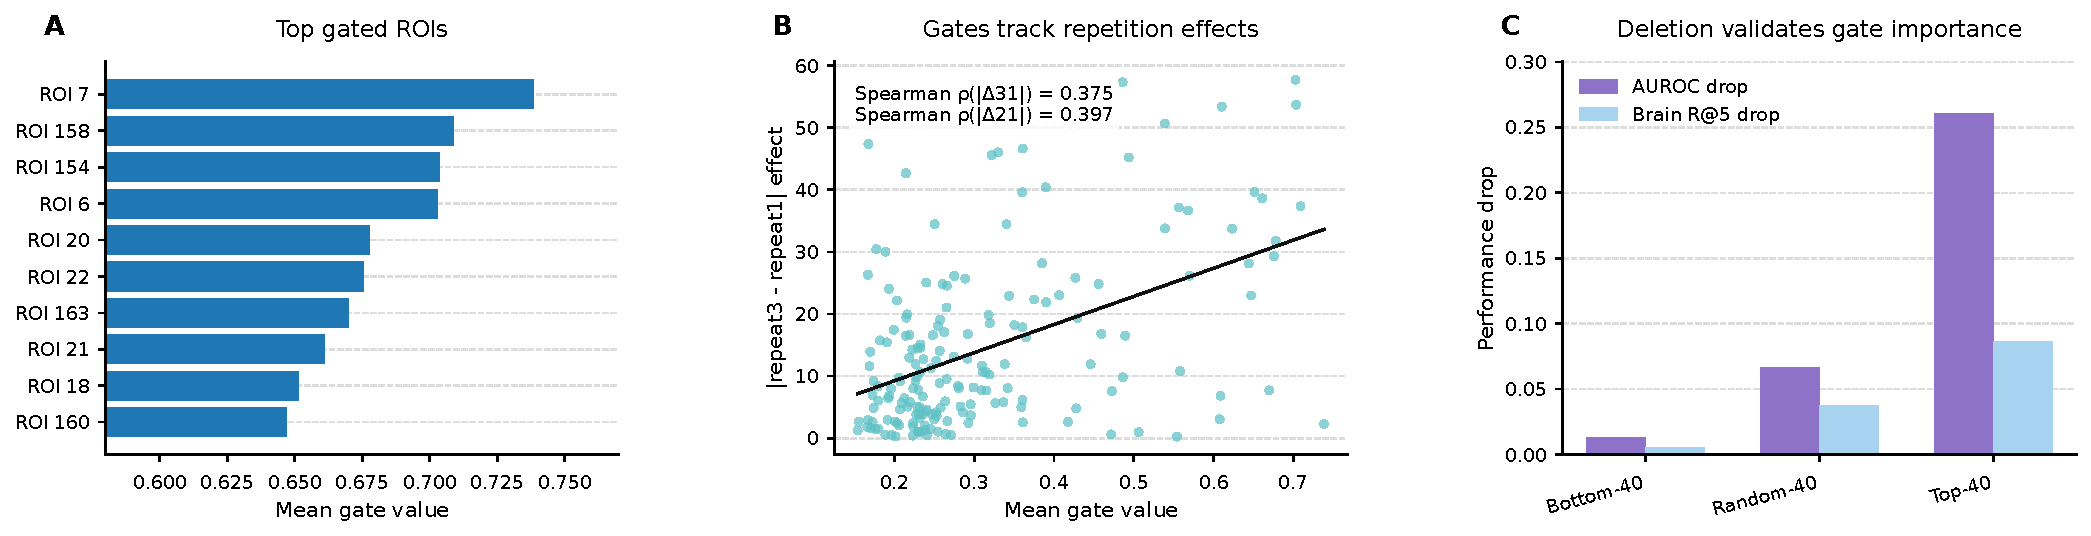
\includegraphics[width=0.98\linewidth]{figures/gate_interpretability.pdf}%
  }{%
    \figtodo{Upload/update \texttt{figures/gate\_interpretability.pdf}: top gated ROIs, gate-vs-repetition scatter, and gate deletion curves.}%
  }
  \caption{Gated-model interpretability. Learned gates are stable and functionally important under ROI deletion tests; confound-controlled analyses motivate cautious interpretation of raw gate--repetition correlations.}
  \label{fig:gates}
\end{figure}

\section{Error Analysis}

Per-subject results show that gated ReGraph+CLIP is strongest on most folds, while fold\_07 remains the hardest held-out subject across all models. Image difficulty analysis covered 766 images. Mean same-image similarity is 0.9274, with standard deviation 0.0077 and range 0.8954 to 0.9451. A fold-level QC audit suggests that fold\_07 is not a simple sample-count artifact: it has the same number of held-out test sequences as folds 01, 02, and 05, but has low repeat reliability, weak raw same/different pair separability, and the lowest raw same-minus-different correlation gap.

\begin{table}[!htbp]
  \centering
  \caption{Fold-level robustness diagnostic for the final gated model. Mean repeat correlation is the average within-subject correlation across repeat pairs in the held-out subject's strict T=3 test sequences. Raw pair AUROC and raw gap are computed from Pearson correlations between serialized positive and negative test pairs before model inference.}
  \label{tab:fold_difficulty}
  \scriptsize
  \setlength{\tabcolsep}{3.5pt}
  \renewcommand{\arraystretch}{1.12}
  \begin{tabular}{llrrrrrr}
    \toprule
    Fold & Test subj. & Test seq. & Repeat corr. & Raw AUROC & Raw gap & Model AUROC & Brain R@5 \\
    \midrule
    fold\_01 & subj01 & 766 & 0.9107 & 0.6615 & 0.0151 & 0.8387 & 0.0963 \\
    fold\_02 & subj02 & 766 & 0.9057 & 0.6697 & 0.0180 & 0.8440 & 0.0865 \\
    fold\_03 & subj03 & 581 & 0.8898 & 0.6469 & 0.0166 & 0.8488 & 0.1279 \\
    fold\_04 & subj04 & 515 & 0.8832 & 0.6919 & 0.0188 & 0.8710 & 0.1439 \\
    fold\_05 & subj05 & 766 & 0.8997 & 0.6824 & 0.0193 & 0.8783 & 0.1113 \\
    fold\_06 & subj06 & 581 & 0.8779 & 0.6486 & 0.0169 & 0.8306 & 0.1038 \\
    fold\_07 & subj07 & 766 & 0.8690 & 0.6296 & 0.0144 & 0.7111 & 0.0374 \\
    fold\_08 & subj08 & 515 & 0.8524 & 0.6158 & 0.0180 & 0.7848 & 0.0893 \\
    \bottomrule
  \end{tabular}
\end{table}

Fold\_07 is therefore not a simple sample-size artifact: it has 766 test sequences, matching folds 01, 02, and 05. Its mean repeat correlation is low and its brain retrieval is the weakest, but fold\_08 has even lower repeat correlation while performing better. Raw same/different separability is more aligned with fold-level AUROC than sequence count, but it still does not fully explain the fold\_07 failure mode. We therefore treat fold\_07 as evidence of a remaining subject-specific robustness or calibration challenge.

\begin{figure}[!htbp]
  \centering
  \IfFileExists{figures/per_subject_performance.pdf}{%
    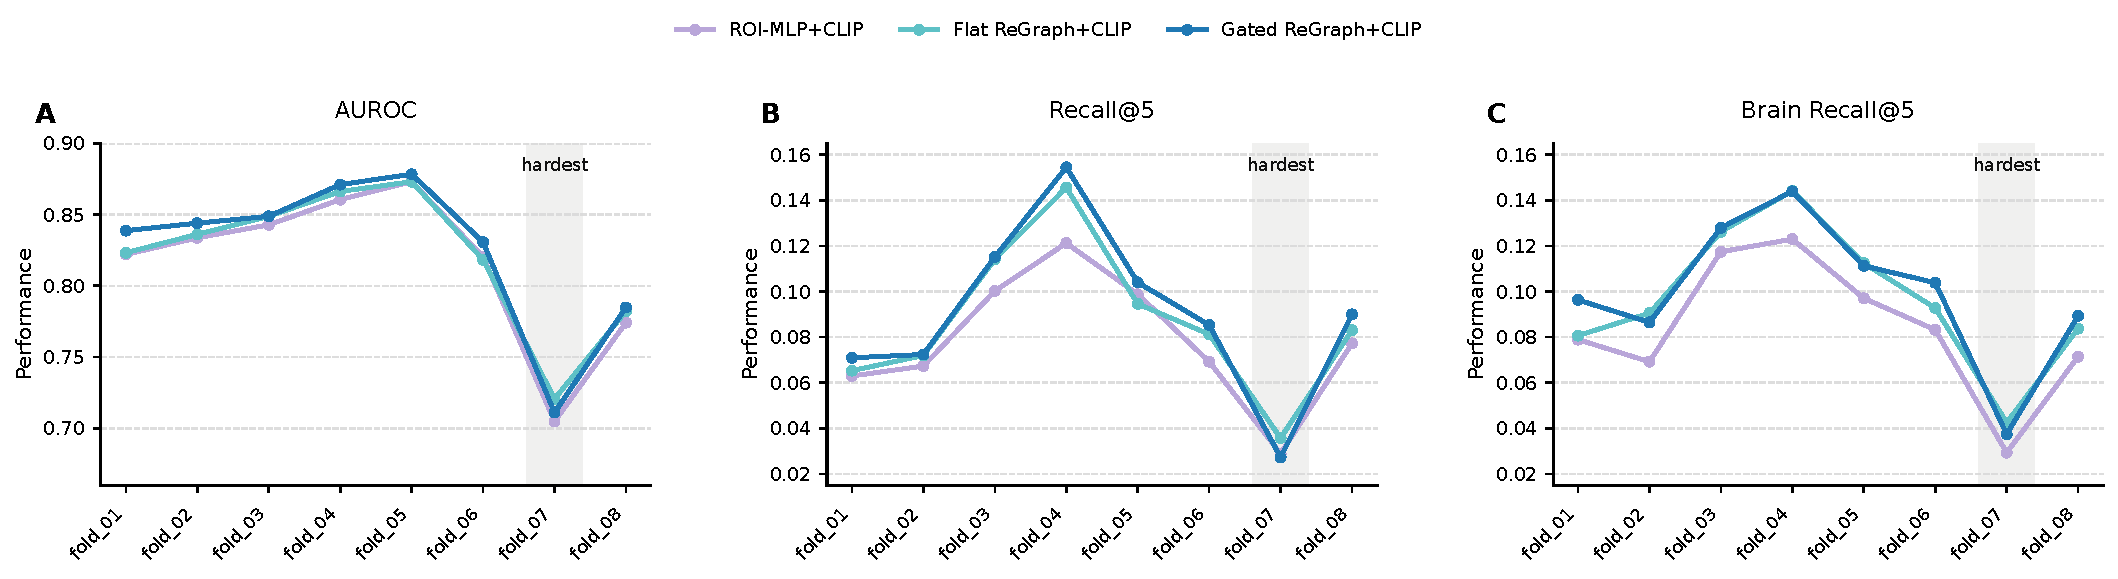
\includegraphics[width=0.98\linewidth]{figures/per_subject_performance.pdf}%
  }{%
    \figtodo{Upload/update \texttt{figures/per\_subject\_performance.pdf}: per-fold/per-subject performance, highlighting fold\_07.}%
  }
\caption{Per-subject cross-subject matching performance.
}
  \label{fig:per_subject}
\end{figure}

\section{Neuroscientific Interpretation and Testable Predictions}
\label{sec:neuro_interpretation}

Our project is not only a graph-learning benchmark. The main scientific goal is to ask whether repeated natural-image fMRI responses contain a shared, image-driven brain graph structure that can be recovered across subjects. In this section, we summarize what our results suggest for visual neuroscience and how they relate to existing findings on repetition effects, representational similarity, and cross-subject neural alignment.

\subsection{Why cross-subject brain graph matching is meaningful}

The central neuroscience question is whether different subjects exhibit a common brain response structure when viewing the same natural image. In our formulation, each trial-level response is a graph over fixed HCP-MMP ROIs, and the model must retrieve the same image or corresponding brain response from other subjects. This task is stricter than within-subject repeat matching: it requires the model to remove subject-specific variability and preserve the common image-driven component of the response.

This formulation is related to several existing ideas in visual neuroscience. First, repeated stimulus presentations are known to produce repetition-related changes in fMRI responses, often discussed under repetition suppression or fMRI adaptation \citep{grill2001fmri,henson2003repetition,grill2006repetition,krekelberg2006adaptation}. Second, representational similarity analysis (RSA) treats neural response patterns as representational objects and compares their similarity structure across stimuli, brain regions, subjects, or models \citep{kriegeskorte2008rsa}. Third, naturalistic fMRI studies have shown that subjects can share stimulus-locked response structure during natural viewing, motivating intersubject correlation and shared-representation analyses \citep{hasson2004isc,haxby2011hyperalignment,nastase2019isc}. Our work combines these ideas in a graph-learning setting: we ask whether a fixed-order brain graph encoder aligned with image embeddings can learn a subject-invariant representation of natural-image responses.

\begin{figure}[!htbp]
  \centering
  \IfFileExists{figures/natural_scene_two_stimuli_repeat_maps_left_lateral_large.png}{%
    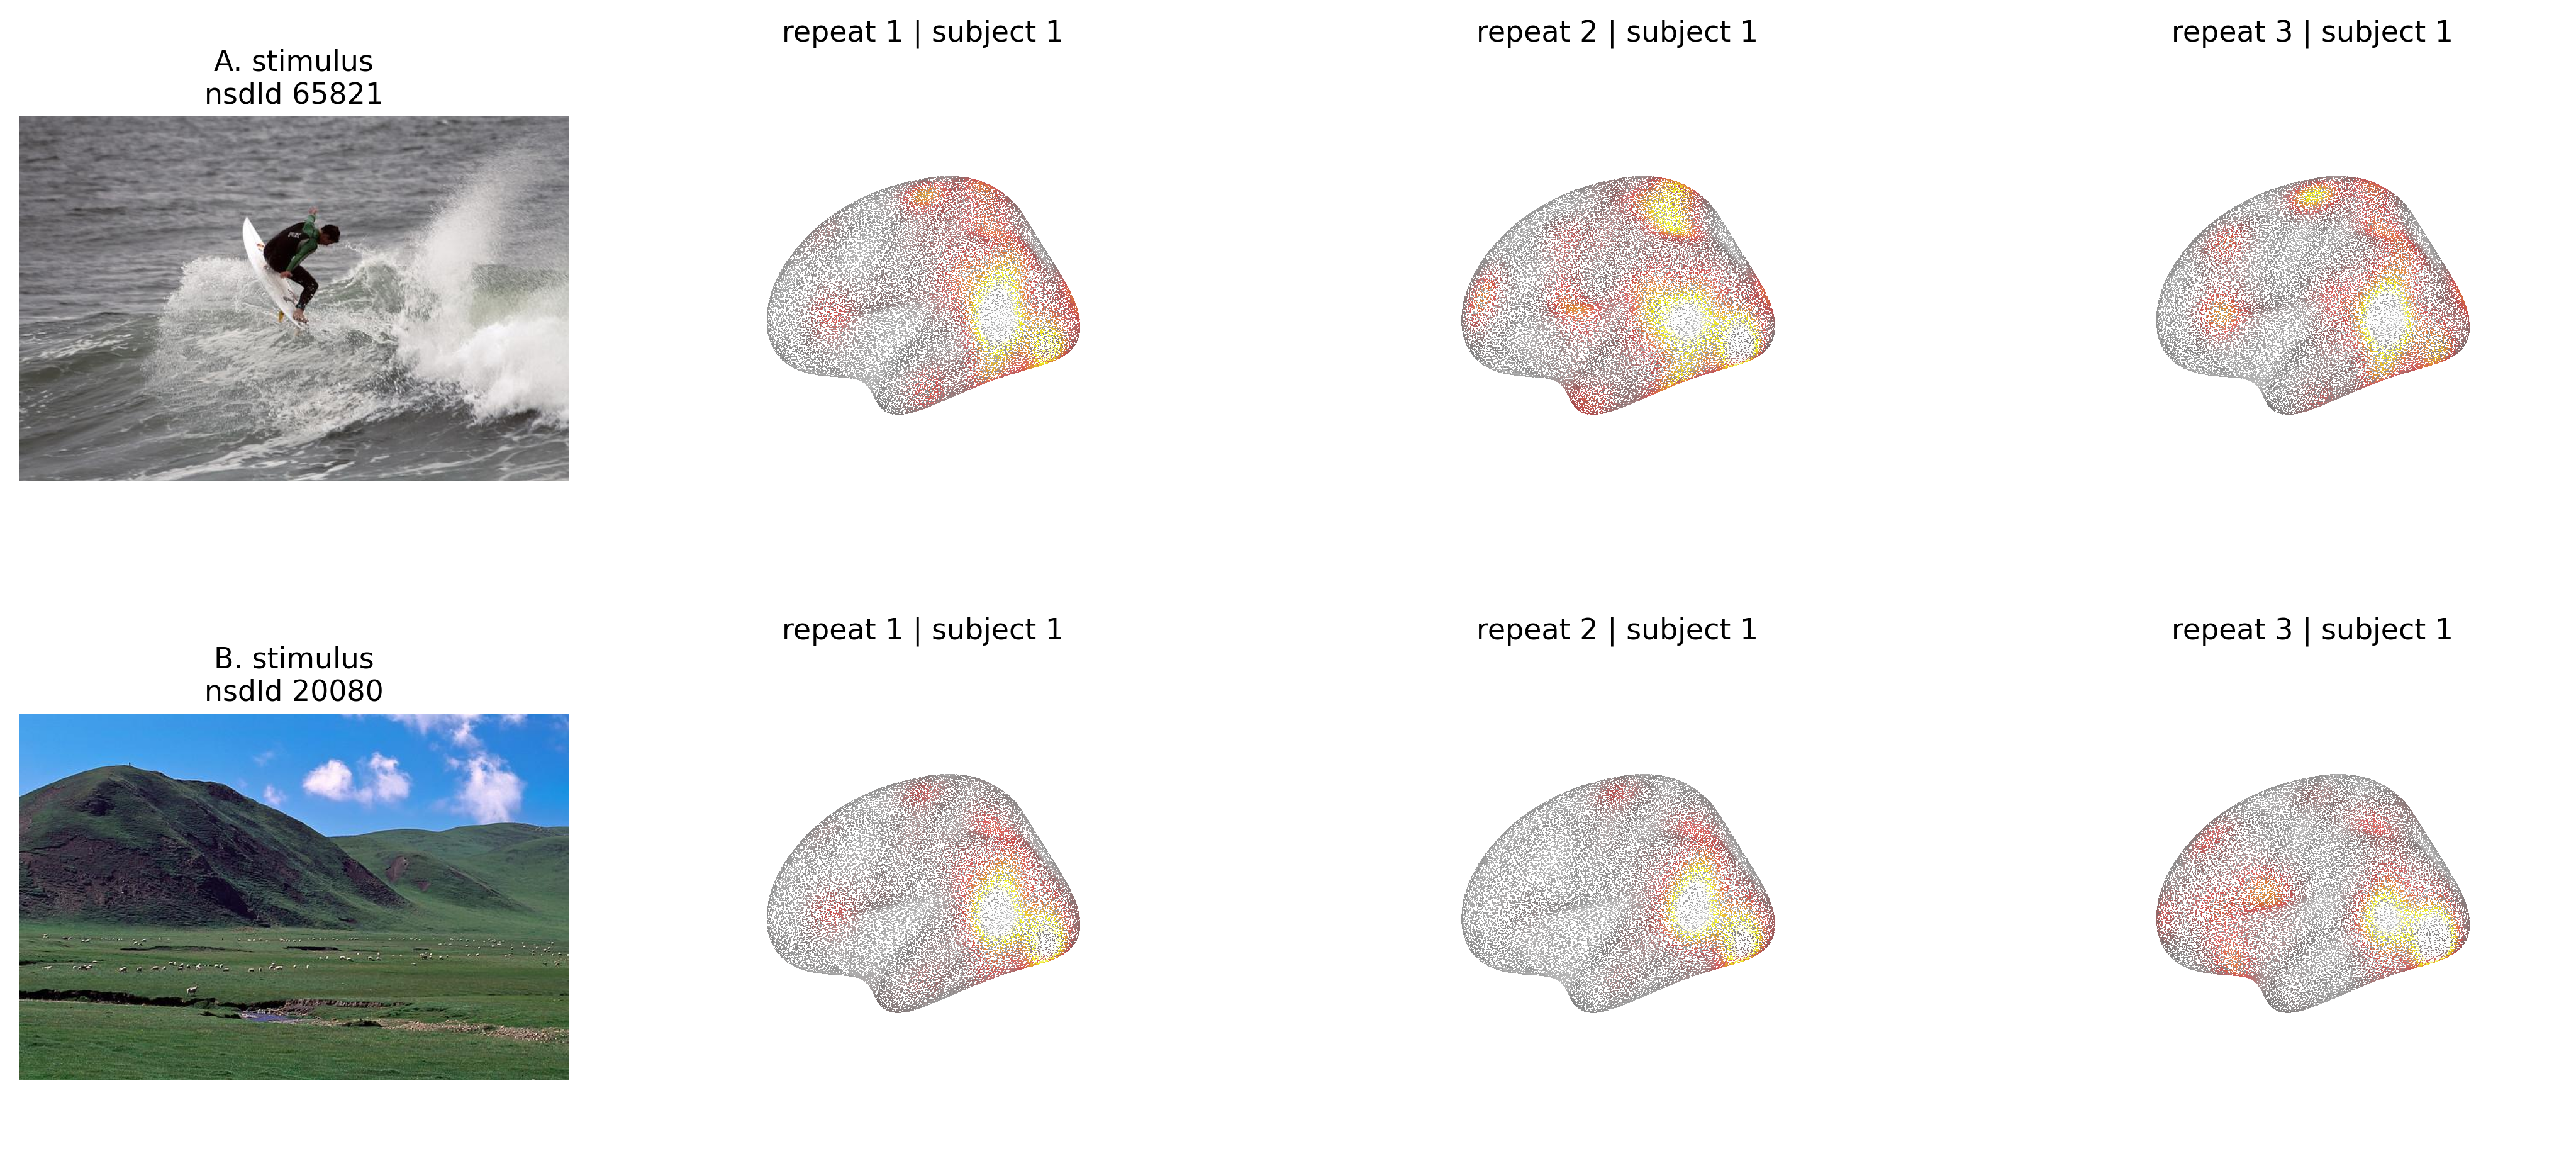
\includegraphics[width=0.98\linewidth]{figures/natural_scene_two_stimuli_repeat_maps_left_lateral_large.png}%
  }{%
    \figtodo{Upload/update \texttt{figures/stimulus\_brain\_reaction\_examples/nsdid9048\_delta31\_cortical\_change.pdf}: example stimulus with cortical map of $|\mathrm{repeat3}-\mathrm{repeat1}|$ response change, formatted like the nsdId 9048 example.}%
  }
  \caption{
Example stimulus-level repeat responses.
Two representative natural-scene images are shown with left-lateral cortical visualizations of the corresponding ROI response maps across repeat1, repeat2, and repeat3 for subject 1.
}
  \label{fig:stimulus_reaction_example}
\end{figure}

\subsection{Our findings align with known repetition and visual-representation effects}

Our first neuroscience finding is that repeated viewing produces measurable ROI-level changes. Across 180 HCP-MMP ROIs, 41 ROIs show FDR-significant repeat2--repeat1 effects and 56 ROIs show FDR-significant repeat3--repeat1 effects. The real mean absolute repetition changes are much larger than shuffled repeat-label nulls. This is consistent with the broad repetition-suppression/adaptation literature, which shows that repeated visual stimuli can change response magnitude in visual cortex \citep{grill2001fmri,henson2003repetition,grill2006repetition,krekelberg2006adaptation}. Importantly, we do not claim that our effects are purely repetition suppression. In natural-image fMRI, repeated responses may reflect a mixture of adaptation, familiarity, attention, memory, session dynamics, and measurement noise. Our contribution is to show that these repeat-related changes are measurable in atlas ROI graph representations and can be used to define graph-learning tasks.

Our second finding is that same-image repeated graphs are more similar than different-image controls. The same-image similarity gaps are consistent across repeat pairs: repeat1--repeat2, repeat1--repeat3, and repeat2--repeat3. This matches the representational similarity view that neural response patterns can preserve stimulus identity even when response magnitude changes \citep{kriegeskorte2008rsa}. In our setting, the graph embedding should preserve the image-specific component across repetitions while becoming invariant to subject-specific and session-specific variation.

Our third finding is that the model's top gated ROIs are concentrated in visual cortex. The strongest gated ROIs map primarily to HCP-MMP visual areas, including V8, V4, V3CD, VMV2/VMV3, LO1/LO2, PIT, VVC, and FFC. These areas span early/intermediate visual cortex, lateral occipital object/shape regions, and ventral-stream high-level visual regions. This is neurobiologically plausible for natural-image retrieval because the ventral visual stream and lateral occipital cortex are strongly involved in object, scene, face, and image-level visual representation \citep{malach1995loc,kanwisher1997ffa,grill2014visual}. The gate analysis therefore supports the idea that ReGraph-VLM is not relying on arbitrary cortical parcels, but instead emphasizes visually meaningful ROIs.

\begin{table}[!htbp]
  \centering
  \caption{
  Top gated ROIs and approximate HCP-MMP visual-area interpretations.
  }
  \label{tab:top_gated_roi_names}
  \scriptsize
  \setlength{\tabcolsep}{4pt}
  \renewcommand{\arraystretch}{1.15}
  \begin{tabularx}{\linewidth}{r l X X}
    \toprule
    ROI ID & HCP-MMP & Region & Broad role \\
    \midrule
    7   & V8   & Ventral visual cortex & Color/form and high-level visual processing \\
    158 & V3CD & Lateral/dorsal occipital cortex & Dorsal visual-complex processing \\
    154 & VMV3 & Ventromedial visual cortex & Ventral visual stream \\
    6   & V4   & Intermediate visual cortex & Color/form processing \\
    20  & LO1  & Lateral occipital cortex & Object and shape processing \\
    22  & PIT  & Posterior inferotemporal cortex & High-level object representation \\
    163 & VVC  & Ventral visual complex & High-level ventral visual representation \\
    21  & LO2  & Lateral occipital cortex & Object and shape processing \\
    18  & FFC  & Fusiform face complex & Face/object-related ventral representation \\
    160 & VMV2 & Ventromedial visual cortex & Ventral visual stream \\
    \bottomrule
  \end{tabularx}
\end{table}

\subsection{What ReGraph-VLM adds beyond descriptive neuroscience}

Traditional repetition analyses often ask whether a brain region changes its mean response across repeated stimuli. Our graph-VLM setting asks a different question: whether repeated and cross-subject responses can be mapped into a shared embedding space that supports image retrieval. The model is successful only if it preserves image identity across people. This makes the learned representation useful for testing subject-invariant visual encoding.

The current results support three claims. First, Gated ReGraph-VLM improves cross-subject same-image retrieval over ROI-MLP+CLIP and flat ReGraph+CLIP, suggesting that fixed-order ROI graph modeling adds value beyond non-graph ROI features. Second, graph-only gated ReGraph performs reasonably on brain-brain matching but has near-chance image/brain retrieval, showing that image alignment is necessary for connecting brain graphs to visual stimuli. Third, held-out-image experiments show that real CLIP embeddings improve image/brain retrieval over random image anchors, suggesting that semantic image structure matters for unseen-image retrieval.

This gives a stronger scientific role to the VLM branch. CLIP is not used simply as a classifier. Instead, it provides a visual-semantic coordinate system in which brain graph embeddings can be aligned with image structure. This is related to recent fMRI-to-image retrieval and reconstruction work that maps brain activity into multimodal latent spaces \citep{scotti2023mindeye}. Our contribution differs by using atlas ROI graphs and fixed-order graph transformers rather than only voxel-vector encoders.

\subsection{Predictions from the model}

The model generates several testable predictions for future neuroscience studies. First, the highly gated ROIs should carry more cross-subject image-retrieval information than low-gated ROIs, a prediction already supported computationally by the ROI deletion test. Second, because mean gate values correlate with independent repetition-effect magnitudes, the same visual ROIs emphasized by the model should show stronger repeat-related modulation in independent repeated-image fMRI datasets. Third, real visual-semantic embeddings should generalize better than random image anchors for unseen-image retrieval, consistent with our held-out-image results where random embeddings remain competitive for pair discrimination but fail on image/brain retrieval. Finally, cross-subject retrieval difficulty should be predictable from subject-level neural stability measures, such as same-image repeat similarity or response reliability; this may explain why fold\_07 is consistently harder across models. These predictions can be evaluated in future work using independent natural-image fMRI datasets, controlled repeat-session designs, and stronger session-matched analyses.

\subsection{Limitations}

The current analyses support model-based hypotheses, not causal neural claims. The learned gates indicate which ROIs are useful for the model, and deletion tests show that those ROIs are functionally important for model performance. However, this does not prove that those regions are causally necessary for human perception or familiarity. Similarly, the cortical maps of repeat3--repeat1 change show structured response differences, but they do not by themselves distinguish adaptation, memory, attention, or session effects. The contribution of this work is to provide a graph-VLM framework that generates testable hypotheses about cross-subject visual brain representations and identifies candidate ROIs for future controlled neuroscience studies.

\section{Discussion}
\label{sec:discussion}

This project began with a simple question: can standard brain graph neural networks decode natural-image fMRI responses from atlas ROI graphs? The static 766-way image-classification experiments showed that the atlas graph pipeline was technically feasible, but also revealed that this initial task was not the right scientific target. ROI MLP baselines were stronger than GCN, GAT, and BrainGNN, and increasing node-feature dimensionality with hand-crafted statistics or PCA did not produce a robust graph advantage. This negative result was useful because it pushed the project toward a more neuroscience-grounded formulation based on repeated natural-image responses.

The repetition/familiarity analyses established that the dataset contains meaningful neural structure. Repeated presentations produced measurable ROI-level response changes, and same-image repeated graphs were consistently more similar than different-image controls. These findings align with prior work on repetition suppression, fMRI adaptation, and representational similarity analysis \citep{grill2001fmri,henson2003repetition,grill2006repetition,krekelberg2006adaptation,kriegeskorte2008rsa}. However, our first-vs-repeated classification diagnostic also showed that simple repeat-state prediction is strongly confounded by session/order structure: a session-only baseline outperformed brain-feature models. Therefore, the final task was reframed as cross-subject same-image graph matching, which asks whether the model can recover the shared image-driven component of brain responses across different people.

The main result is that Gated ReGraph-VLM improves cross-subject brain graph matching and retrieval over strong baselines. ROI-MLP+CLIP is a strong non-graph control, flat ReGraph+CLIP is a strong fixed-order graph transformer baseline, and the newly added task-matched component baselines test recent directions in shared fMRI-to-image mapping, subject-conditioned universal encoding, and subject-adversarial training. The closest component baseline is the MindLink-style subject-adversarial ROI-MLP, but it remains below Gated ReGraph-VLM on AUROC, retrieval R@5/MRR, and brain retrieval.

The most important update is that the graph contribution must be framed carefully. The no-adjacency gated ROI Transformer is statistically tied with the final BNT/ReGraph ROI-token variant, while ROI-order shuffling collapses performance and learned gate controls reduce performance. Static adjacency perturbations and learned edge-bias follow-ups do not show a clear advantage over no adjacency. Therefore, the current result should not be claimed as evidence that fixed Pearson adjacency is responsible for the gain. The stronger and safer claim is that fixed anatomical ROI-token layout, learned transformer interactions, gated ROI-preserving readout, and CLIP alignment improve cross-subject retrieval.

The VLM component also plays an important role. The graph-only gated model can perform brain-brain matching, but image and brain retrieval are near chance without CLIP alignment. At the same time, random image-embedding controls indicate that the auxiliary embedding loss can also act as a regularizer or image-anchor constraint. The held-out-image analysis clarifies this issue: random embeddings remain competitive for pair discrimination but collapse on image/brain retrieval, whereas real CLIP embeddings preserve semantic retrieval performance. Thus, the most careful interpretation is that image-alignment supervision improves embedding geometry in general, while real CLIP semantics are especially important for generalizing image/brain retrieval to unseen images.

Exploratory external smoke tests on public visual-ROI summaries from CNeuroMod-THINGS, BOLD5000, THINGS-fMRI, and LAION-fMRI further clarify the scope of the claim. These datasets show above-chance cross-subject same-image signal outside NSD, but the compact visual-ROI summaries do not reproduce a consistent gated-transformer advantage over ROI-MLP. This is useful stress-test evidence, not a full external replication. It suggests that the main NSD result should be framed around the validated HCP-MMP ROI-token setting, while future external work should use trial-wise atlas-level beta maps rather than only public visual-localizer or compact table-format visual ROI summaries.

A second contribution is interpretability. The gated readout provides a model-native ROI importance signal. The top gated ROIs are concentrated in visual cortex, including early/intermediate visual areas, lateral occipital regions, and ventral-stream regions such as V8, V4, LO1/LO2, PIT, VVC, FFC, and VMV areas. The gate values are stable across folds and seeds, and deletion tests show that removing highly gated ROIs damages model performance much more than removing random or property-matched control ROIs. At the same time, confound-controlled analysis shows that the raw gate--repetition correlation is largely explained by ROI reliability and response properties. Therefore, gates should be interpreted as model-level evidence for reliable, visually informative ROIs, not as causal proof of repetition-specific neural mechanisms.

This work has several limitations. First, the analysis uses atlas-level ROI summaries rather than full voxel patterns, so fine-grained within-ROI information is compressed. Second, although the cross-subject results are strong, the main dataset contains only eight subjects. Our external visual-ROI smoke tests are useful feasibility checks, but full external validation on independent trial-wise atlas-ROI beta maps remains needed for broader generalization. Third, repeat-related effects in NSD can reflect adaptation, familiarity, memory, attention, and session dynamics; our model identifies useful response structure but does not isolate these mechanisms causally. Fourth, the final cross-subject pair tensors are exactly anchor-side session/order matched, and both eval-only and retrained single-reference controls support the fixed ROI-token conclusion; however, the primary benchmark still uses averaged references, and the retrained single-reference control again shows that explicit fixed adjacency is tied with no adjacency rather than providing a separate gain. Fifth, explicit fixed adjacency does not explain the main gain, so future graph-specific work should test stronger learned edge mechanisms or biologically grounded module priors. Finally, although real CLIP embeddings improve held-out image retrieval, the role of semantic structure versus auxiliary image anchoring should be further tested using additional VLMs, controlled prompt sets, and semantically matched hard negatives.

Overall, the results support a stronger conclusion than simple fMRI graph classification. Gated ReGraph-VLM learns a subject-invariant, image-aligned brain graph representation that improves cross-subject retrieval and produces interpretable ROI-level hypotheses. The project therefore contributes both a graph-VLM method for visual fMRI and a neuroscience framework for studying repeat-stable natural-image representations across subjects.

\section{Conclusion}
\label{sec:conclusion}

We presented \textbf{Gated ReGraph-VLM}, a fixed-order brain graph--vision model for repeated natural-image fMRI. The model encodes HCP-MMP ROI response graphs with a BNT-style ROI transformer, applies a gated anatomy-preserving readout, and aligns brain graph embeddings with CLIP image embeddings. After initial static image-classification experiments showed that standard graph baselines were insufficient, we reformulated the task as cross-subject same-image brain graph matching and retrieval. In this setting, Gated ReGraph-VLM improves over ROI-MLP+CLIP and flat ReGraph+CLIP in the main all-fold and hard-negative settings, and it is strongest among real-CLIP models for held-out-image image/brain retrieval. It also remains stronger than newly added task-matched decoding component baselines inspired by MindEye2, UMBRAE, and MindLink, with the closest competitor being a subject-adversarial ROI-MLP that still underperforms on every key metric.

Beyond predictive performance, the model provides neuroscience-relevant insights. Repeated natural-image responses show significant ROI-level changes and strong same-image representational stability. The learned gates concentrate in visual ROIs and are functionally important under deletion tests. The new confound-controlled analysis makes this interpretation more precise: gate values should be treated as model-level ROI importance signals that emphasize reliable, visually informative cortex, not as causal evidence for repetition-specific neural mechanisms.

The final contribution is therefore twofold. Methodologically, ReGraph-VLM shows that fixed anatomical ROI-token modeling, gated ROI-preserving readout, and image alignment improve cross-subject brain-image retrieval beyond non-graph, standard graph, and task-matched decoding component baselines. Scientifically, it provides a framework for studying how repeated natural images are represented across subjects in visual cortex, and it generates testable predictions about which ROIs should carry cross-subject image-retrieval information in future fMRI experiments.

\section{Limitations}
\label{sec:limitations}

This work has several limitations. We use atlas-level ROI graph features rather than full voxel-level response patterns, which improves interpretability but may discard fine-grained image-specific information. The main dataset contains only eight subjects. We added external smoke checks on public visual-ROI summaries from CNeuroMod-THINGS, BOLD5000, THINGS-fMRI, and LAION-fMRI, but these are not full HCP-MMP external validations; broader validation on independent trial-wise atlas-ROI beta maps remains needed. Repetition effects in NSD may reflect adaptation, memory, attention, session structure, or scanner variability, so we avoid interpreting repeat-state decoding as a clean novelty/familiarity measure. The final cross-subject pair tensors are exactly anchor-side session/order matched, and both eval-only and retrained single-reference controls now support the fixed ROI-token conclusion; however, the primary benchmark still uses averaged references and fold\_07 remains an unresolved robustness case. Although held-out-image experiments support the value of real CLIP embeddings for image/brain retrieval, shuffled and random embedding controls suggest that part of the auxiliary image-alignment objective may also act as regularization. Finally, the learned gates provide model-level explanations rather than causal neuroscience evidence; future work should test voxel-level features, stronger session controls, edge-level mechanisms, and external dataset generalization.

\bibliographystyle{plainnat}
\bibliography{references}

\end{document}
